\chapter{Differential Geometry: Distance and Direction in Curved Spaces}

\section{That Strange Detour on the Map}

Open a world map and find Beijing and San Francisco. Imagine you are an airline pilot planning the most fuel-efficient route between them. Intuition says to join the cities with a ruler and fly straight along that line.

Real flights do something else. From Beijing they head northeast, passing over northeastern China and Russia's Far East, near the Aleutian Islands, before turning southeast towards San Francisco. On the map the route bulges conspicuously northward. Airlines burn tens of thousands of tonnes of fuel each year; they would not take a detour without reason.

Consider an older example. Fifteenth-century navigators already knew that sailing due west along one latitude was not the quickest route to a distant port. Clever captains first headed towards higher latitudes, then turned back. Sailors called this "great-circle sailing". They did not know why it worked, only that it was faster.

This leaves us with a question:

\begin{center}
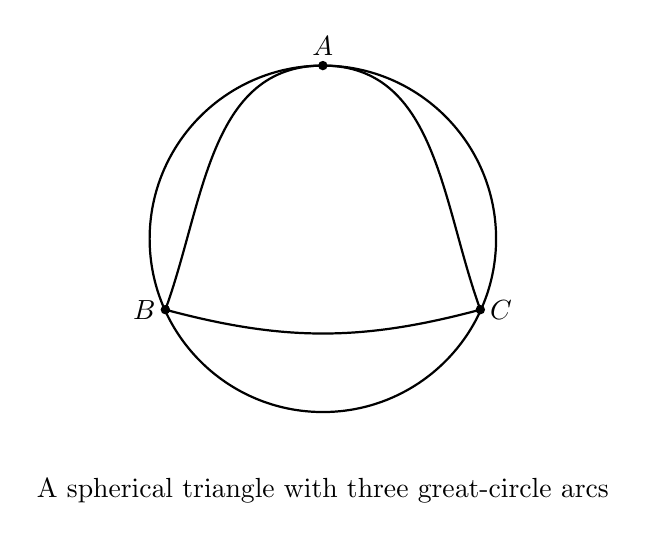
\begin{tikzpicture}
  \draw[thick] (0,0) circle (2.2);
  \coordinate (P) at (0,2.2);
  \coordinate (A) at (-2.0,-0.9);
  \coordinate (B) at (2.0,-0.9);
  \draw[thick] (A) to[out=70,in=180] (P);
  \draw[thick] (P) to[out=0,in=110] (B);
  \draw[thick] (A) to[out=-15,in=195] (B);
  \fill (P) circle (0.06) node[above] {$A$};
  \fill (A) circle (0.06) node[left] {$B$};
  \fill (B) circle (0.06) node[right] {$C$};
  \node at (0,-3.2) {A spherical triangle with three great-circle arcs};
\end{tikzpicture}
\end{center}

On a curved surface, what does "straight" mean? How should distance be measured and direction described? These sound like questions for pilots and captains, but they lead to differential geometry, a deep subject studying lengths, angles, and shapes in curved spaces. Early in the twentieth century, it became Einstein's language for gravity. We will travel from a bending flight route to curved spacetime.

\section{When Intuition Fails: Orange Peel That Will Not Lie Flat}

The first natural response to spherical distance is to flatten the sphere. Then a ruler can measure it: easy.

Try this at home. Peel an orange, keeping the peel as intact as possible, and attempt to lay it flat without gaps or overlaps. You cannot: either the edges split or the middle bulges. Compare a flat sheet of paper rolled effortlessly into a cylinder. Unroll it and it returns unchanged, without tears or wrinkles.

This failed kitchen experiment reveals a deep dividing line: cylinders and planes are relatives, deformable into one another without stretching; spheres and planes are not. Every flat map of a sphere must pay a price in distortion.

How large a price? On the familiar Mercator world map, Greenland looks about as large as Africa, though Africa is actually about fourteen times larger. The map is not mistaken; it simply cannot preserve all lengths, angles, and areas. Some maps preserve angles at the expense of areas; others preserve areas at the expense of shapes. Mathematicians have proved that a flat spherical map preserving distance, angle, and area simultaneously cannot exist.

\begin{fanli}
"Flatten the sphere before measuring, and surely we are back in plane geometry?" This plausible plan fails. A sphere cannot be flattened without stretching or tearing, so spherical geometry is not plane geometry in disguise: it has its own laws. Likewise, following a latitude circle is not the shortest route from Beijing to San Francisco. Except for the equator, latitude circles are not great circles, so following one is a detour.
\end{fanli}

Our first attempt failed but pointed the way. Stop trying to turn surfaces into planes; learn to live inside their geometry, like an ant on a sphere understanding its world through measurements underfoot, without stepping outside.

\section{Coordinates on a Surface: An Atlas Is Enough}

The ant needs no perfect map of the entire sphere, only an atlas. Each page maps a small region, approximately planar. Neighbouring pages overlap, assigning two coordinate systems to the same place, with a conversion rule translating between them.

This idea is important enough to name.

\begin{dingyi}
If a small surface region corresponds one-to-one and sufficiently smoothly to a disc in the plane, we assign it planar coordinates $(u,v)$ and call it a \textbf{coordinate chart}. Charts covering the whole surface, with coordinate conversions on their overlaps, form a \textbf{coordinate atlas}.
\end{dingyi}

You have something similar at home. No world map portrays Earth perfectly, but a regional atlas works well: one province per page, with overlaps linking the pages. Likewise, a single chart cannot cover the globe without trouble, particularly at the poles, but two or three suffice. The key is that lengths, angles, and areas must be computable in each chart and agree on overlaps. Then the ant has a complete geometry without needing to know that the sphere sits inside three-dimensional space.

Looking only from within a surface is the intrinsic viewpoint. The contrasting external view makes a sphere's curvature immediately visible in three-dimensional space. A turning point in mathematics came with the recognition that intrinsic geometry can stand alone: inhabitants can measure whether their surface curves, and how much, without going outside. A mathematician called the central result the "remarkable theorem": intrinsic curvature belongs to the surface itself. Flattening and rolling that preserve intrinsic curvature cannot fool a measurer living on the surface.

\section{Tangent Planes and Tangent Vectors: Finding Your Footing}

Before an ant can crawl on a sphere, it must ask what direction means.

On a plane, direction is an arrow, a vector. But where does an arrow on a sphere point? To lie on the sphere, it must curve with the surface, no longer resembling a familiar vector. Instead, place an infinitely thin flat board at a point $P$, touching the sphere only at $P$ and suspended elsewhere. This is the \textbf{tangent plane} at $P$.

\begin{center}
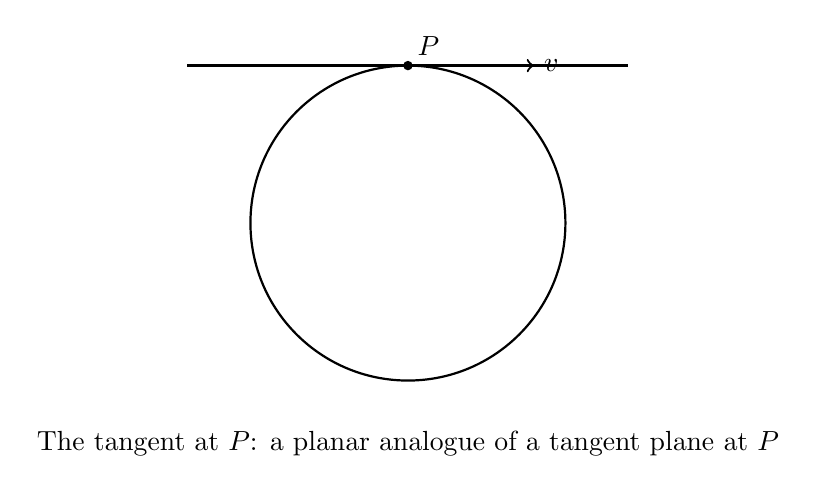
\begin{tikzpicture}
  \draw[thick] (0,0) circle (2);
  \draw[thick] (-2.8,2) -- (2.8,2);
  \fill (0,2) circle (0.06) node[above right] {$P$};
  \draw[->,thick] (0,2) -- (1.6,2) node[right] {$v$};
  \node at (0,-2.8) {The tangent at $P$: a planar analogue of a tangent plane at $P$};
\end{tikzpicture}
\end{center}

\begin{dingyi}
A surface's \textbf{tangent plane} at $P$ touches the surface there and contains all its directions at that point. A vector in this plane starting at $P$ is a \textbf{tangent vector} to the surface at $P$.
\end{dingyi}

Tangent vectors solve a real difficulty: they make taking a small step in a particular direction precise. The step itself curves along the surface, but when infinitesimal it differs negligibly from a straight segment in the tangent plane: the error shrinks faster than the step length. This is the role of "differential": infinitesimally locally, a curved surface and its tangent plane are the same.

You live inside this approximation every day. Earth has radius about $6371$ kilometres and the ground beneath you is spherical, yet across a few dozen metres its deviation from a tangent plane is only millimetres. Building houses and playing football can treat it as flat. Locally planar, globally curved: remember this phrase, which will return in a more important role.

\begin{shuyu}{Tangent plane}
\textbf{Intuition}: Gently touch a basketball with a glass plate at one point. The plate lies in the tangent plane. Touch elsewhere and its orientation changes.

\textbf{Formal definition}: The tangent plane at a surface point is spanned by the tangent directions of all smooth curves through that point.

\textbf{Example}: The small patch of ground where you stand approximates Earth's tangent plane beneath your feet; a spirit level measures it.
\end{shuyu}

\section{Curvature: Measuring How Much Things Bend}

With tangent planes, we can quantify bending. The idea is direct: the faster surface points depart from the tangent plane, the more strongly the surface bends there.

Start with a one-dimensional analogy. A circle of radius $r$ bends equally everywhere; its curvature is defined as $1/r$. Smaller radius means sharper bending. As radius tends to infinity, curvature tends to zero and the circle becomes a straight line, whose curvature is zero. For $r=2$, curvature is $1/2$; for $r=100$, it is just $0.01$, hardly noticeable over a short walk.

Surfaces are more complicated: at one point, different directions may bend differently. A sphere bends equally in every direction. For radius $R$, every directional cross-section is a great circle of radius $R$, with curvature $1/R$. A cylinder differs: across its circular direction the section is a circle of radius $R$, curvature $1/R$; along a generator, the vertical direction, it is a straight line with zero curvature. Multiplying the curvatures in the two extreme directions gives \textbf{Gaussian curvature}. Thus:

\[ \text{Sphere's Gaussian curvature} = \frac{1}{R}\cdot\frac{1}{R} = \frac{1}{R^2}, \qquad \text{Cylinder's Gaussian curvature} = \frac{1}{R}\cdot 0 = 0. \]

At first this seems wrong: a cylinder visibly bends, so why is its Gaussian curvature zero? Recall the orange peel. A cylinder is made by rolling paper without stretching. An ant living on it makes the same measurements as an ant on a plane: its intrinsic geometry is planar. Gaussian curvature measures intrinsic bending, not external appearance. Conversely, a sphere's everywhere-positive $1/R^2$ quantifies why orange peel cannot lie flat. Earth's radius is about $6371$ kilometres, giving surface Gaussian curvature $1/(6.371\times 10^6)^2 \approx 2.5\times 10^{-14}$ per square metre. Tiny but positive, it accumulates to prevent any perfect world map.

A third possibility is a saddle. At its centre, the surface bends downwards fore and aft and upwards side to side. Opposite signs multiply to give negative Gaussian curvature. What happens when such a surface is flattened? Unlike the sphere's shortage of material, which causes splitting, it has too much material, producing wrinkles and overlaps like a wood-ear mushroom. Three signs, three fates: positive curvature splits, zero lies flat, negative wrinkles.

\section{Spherical Triangles: The Angle Sum Rebels}

Among our earliest geometry theorems, one is etched into memory: a triangle's angles sum to $180^\circ$. Now we will watch it fail on a sphere, in a remarkably orderly way.

First define a spherical triangle. Great circles play the role of straight lines: intersections of the sphere with planes through its centre. The equator and complete meridian circles qualify; other latitude circles do not, since their planes miss the centre.

\begin{dingyi}
Choose three points on a sphere not lying on one great circle and join them pairwise with three great-circle arcs. The enclosed figure is a \textbf{spherical triangle}. Its interior angles are the angles between the tangent lines to the meeting arcs at each vertex.
\end{dingyi}

Consider an extreme, beautiful example. Let $A$ be the North Pole and choose equatorial points $B$ and $C$ with longitude difference $90^\circ$. Sides $AB$ and $AC$ follow meridians, while $BC$ follows the equator. At $A$, the meridians meet at their longitude difference, $90^\circ$. At $B$, meridian and equator are perpendicular, giving $90^\circ$; likewise at $C$, $90^\circ$. All three angles are right angles, summing to $270^\circ$, fully $90^\circ$ more than on a plane!

This excess is not error, but area. Early in the nineteenth century, a mathematician proved one of spherical geometry's loveliest formulas:

\begin{dingli}[Area of a spherical triangle]
On a sphere of radius $R$, a spherical triangle with interior angles $A$, $B$, $C$ measured in radians and area $S$ satisfies
\[ S = R^2\,(A + B + C - \pi). \]
In particular, its angle sum exceeds $\pi$, or $180^\circ$, and the excess $A+B+C-\pi$ is proportional to its area.
\end{dingli}

\begin{proof}
The proof has three steps, each visible in a diagram.

\textbf{Step 1: Area of a lune.} Two intersecting great circles divide the sphere into four crescent-shaped regions called lunes. A lune of angle $A$ radians occupies the fraction $A/(2\pi)$ of the sphere: imagine slicing a watermelon by longitude through $2\pi$ radians and taking $A$ radians. Since the whole sphere has area $4\pi R^2$, the lune's area is
\[ 4\pi R^2 \cdot \frac{A}{2\pi} = 2R^2 A. \]
Check: at $A=\pi$, the lune is a hemisphere, and the formula gives the correct area $2\pi R^2$.

\textbf{Step 2: Three pairs of lunes cover the sphere.} Let triangle $T$ have angles $A$, $B$, and $C$. The great circles containing its two sides at $A$ enclose a pair of opposite lunes of angle $A$, each with area $2R^2 A$. Likewise obtain pairs for $B$ and $C$. These six lunes cover the sphere with overlaps: $T$ is covered $3$ times, as is its congruent antipodal triangle, while every other point is covered exactly $1$ time.

\textbf{Step 3: Write the equation.} The total area of the six lunes equals the sphere's area plus $4$ extra copies of $T$: $2$ extra copies of $T$ and $2$ of its antipodal partner:
\[ 2\,(2R^2 A + 2R^2 B + 2R^2 C) = 4\pi R^2 + 4S. \]
Divide by $4R^2$ and rearrange:
\[ S = R^2 (A + B + C - \pi). \]
This completes the proof.
\end{proof}

Check our example: the polar-equatorial triangle has $A=B=C=\pi/2$, sum $3\pi/2$, so $S = R^2(3\pi/2 - \pi) = \pi R^2 /2$. Directly, it occupies one-eighth of the globe: meridians differing by $90^\circ$ select a quarter, then taking the northern half halves that. Its area is $\frac{1}{8}\cdot 4\pi R^2 = \pi R^2/2$, exactly matching.

\begin{tuilun}
No spherical triangle has angle sum exactly $180^\circ$. The greater its excess over $180^\circ$, the larger the triangle. As a triangle shrinks, the excess tends to zero: locally, spherical geometry approaches plane geometry.
\end{tuilun}

This locks in our earlier phrase: locally planar, globally curved. Inhabitants measure curvature through the amount by which angle sums betray the planar rule.

\begin{lianjie}
Recall the planar proof that triangle angles sum to $180^\circ$: it uses the parallel postulate, giving exactly one parallel through an external point. Any two great circles intersect, so spheres have no parallel lines. The postulate fails and the angle-sum theorem changes. No proof went wrong; the geometric stage changed. Historically, two thousand years of doubt and debate about the parallel postulate led mathematicians towards curved-space geometry. Spherical geometry is one legacy of that internal struggle. Next chapter, another familiar certainty---the precise number from a measurement---will likewise change under randomness.
\end{lianjie}

\section{Geodesics: Straightest and Shortest}

Return to the opening question: what does walking straight on a surface mean? With no compass, an ant understands it as never turning left or right, simply crawling in the direction it faces. Such a route is a \textbf{geodesic}.

\begin{shuyu}{Geodesic}
\textbf{Intuition}: A route that does not turn on the surface. Stretch a rubber band between two surface points; its resting path is a geodesic.

\textbf{Formal description}: A geodesic is locally shortest: between any sufficiently close pair of its points, no shorter surface route exists. Equivalently, it proceeds straight along the surface with zero sideways acceleration.

\textbf{Example}: On a sphere, geodesics are great circles. The shortest Beijing--San Francisco route is the shorter arc of the great circle through both cities and Earth's centre.
\end{shuyu}

Why do straightest and shortest coincide? If a route has a turn, cutting the corner shortens it, so a shortest route cannot turn anywhere. Conversely, every small segment of a route that never turns is shortest. On a plane, geodesics are straight lines; on a sphere, great circles. Cut and flatten a cylinder, and its geodesics become straight segments; roll it back and one may become an ascending helix. A helix can therefore be the straightest route, a startling idea at first hearing.

Calculate the saving. Beijing is roughly $40^\circ$ north, $116^\circ$ east; New York roughly $41^\circ$ north, $74^\circ$ west. Their latitudes nearly match and longitudes differ by about $170^\circ$. Flying along latitude, approximately straight on a flat map, follows the $40^\circ$ north circle of radius $R\cos 40^\circ$, with arc length
\[ \frac{170}{360}\times 2\pi R \cos 40^\circ \approx 0.472 \times 2\pi \times 6371 \times 0.766 \approx 14500 \text{ km}. \]
The actual great-circle route is about $11000$ kilometres, saving roughly three thousand five hundred kilometres, more than a Beijing--Urumqi round trip. The curved arc on the map is the sphere's true straight line.

\begin{shiyan}
Find an orange or table-tennis ball, a marker, soft string, and a protractor, or estimate angles if none is available.

Step 1: Mark three points on the ball. Pull the string taut against the surface between pairs and draw three straight routes along it. These are great-circle arcs, or geodesics.

Step 2: Observe the triangle's angles, estimate or measure each, and add them. Larger triangles exceed $180^\circ$ by more; very small ones approach $180^\circ$.

Step 3, for comparison: draw a triangle on paper, roll the paper into a cylinder, then unroll it and measure. The angle sum stays unchanged. Why did the spherical triangle change while the paper triangle did not?
\end{shiyan}

\section{Manifolds: Locally Flat, Globally Full of Possibilities}

We have repeatedly used one pattern: locally planar, globally perhaps very different. Mathematicians made that pattern itself an object of study.

\begin{dingyi}
A space is a \textbf{two-dimensional manifold} if a small neighbourhood of every point corresponds smoothly and one-to-one to a planar disc, so it can be mapped by a chart. Replacing the plane by flat $n$-dimensional space gives an $n$-dimensional manifold.
\end{dingyi}

\begin{shuyu}{Manifold}
\textbf{Intuition}: A manifold is a space coverable by an atlas. Wherever you stand, your surroundings seem flat; only travelling around the world reveals its different global shape.

\textbf{Formal definition}: Every point has a neighbourhood smoothly equivalent to an open disc in flat space, with sufficiently smooth coordinate changes between charts.

\textbf{Example}: A sphere is a two-dimensional manifold, as is a doughnut's surface, the torus. Two crossing planes are not: no neighbourhood of their intersection can be flattened into a disc.
\end{shuyu}

The torus deserves more discussion. Its outside is sphere-like with positive curvature; its inside saddle-like with negative curvature; globally it is a closed manifold without boundary. An ant drawing triangles finds some with sums above $180^\circ$ and others below $180^\circ$, as curvature changes sign with location. More intriguingly, identifying both pairs of opposite sides of a rectangular paper sheet---first making a cylinder, then joining its ends---also gives a torus, yet this paper torus is intrinsically flat. It supports geometry with triangle angles summing exactly to $180^\circ$. One topological shape can carry different geometries. Distinguishing shape from geometry is a starting point of modern geometry.

\begin{table}[h]
\centering
\begin{tabular}{llll}
\toprule
Surface & Triangle angle sum & Geodesics & Flattens without stretching? \\
\midrule
Plane & Exactly $180^\circ$ & Straight lines & Already flat \\
Sphere & Above $180^\circ$; larger excess for larger triangles & Great-circle arcs & No: it splits \\
Cylinder & Exactly $180^\circ$ & Straight when unrolled; possibly helices & Yes \\
Saddle & Below $180^\circ$ & Outward-diverging curves & No: it wrinkles \\
\bottomrule
\end{tabular}
\end{table}

Why lavish such attention on manifolds? Because we ourselves inhabit one. Looking at the universe, we directly experience only a small, approximately flat neighbourhood. Whether the whole is closed or open, flat or curved cannot be seen at a glance. It must be inferred gradually through internal measurements: triangle angles, convergence or divergence of parallel light beams, and counts of distant galaxies. The ant's method for studying a sphere is the astronomer's method for studying the universe.

\section{From Local Geometry to the Stars: A Popular-Science Glimpse}

In 1854, a mathematician's lecture systematically introduced curved spaces of arbitrary dimension: curvature can vary from point to point, lengths and angles depend on a varying metric, and geodesics replace straight lines. At the time, these tools were pure intellectual play, with no known use.

Sixty-one years later, in 1915, Einstein recognised exactly the language he needed. In popular-science terms, general relativity says that what we call gravity is spacetime curvature. Matter and energy curve spacetime, and freely falling objects follow its geodesics. Planets orbit not because invisible ropes pull them, but because they travel straight through curved spacetime. During the 1919 solar eclipse, astronomers observed distant starlight deflected near the Sun by an amount matching the prediction: light followed spacetime geodesics, and the Sun curved that spacetime.

We must honestly mark the boundary: this is a popular analogy. General relativity treats four-dimensional spacetime, three spatial dimensions and one temporal, with geometry intertwined with the passage of time and described by precise equations. A picture of a heavy ball on a rubber sheet cannot capture it. This chapter offers an entrance: curved spaces admit intrinsic measurement, geodesics replace straight lines, and curvature replaces gravity. These are ideas you can now explore directly on a sphere.

\begin{pandeng}
Further signposts: Gaussian curvature and the remarkable theorem; covariant derivatives and parallel transport, describing vectors carried along curves; the Gauss--Bonnet theorem, linking total curvature to hole count and bridging geometry and topology; Riemannian geometry and metric tensors; and eventually formal courses in differential geometry and general relativity. After multivariable calculus and linear algebra, each of these keywords will become accessible.
\end{pandeng}

\begin{toolbox}
New tools from this chapter:

\begin{itemize}
  \item \textbf{Charts and atlases}: Cover a surface with planar coordinate patches and convert on overlaps; geometry need not flatten the surface.
  \item \textbf{Tangent planes and vectors}: All directions at a point form its tangent plane; infinitesimally, plane and surface are indistinguishable.
  \item \textbf{Gaussian curvature}: The product of extreme directional curvatures measures intrinsic bending: positive splits when flattened, zero lies flat, negative wrinkles.
  \item \textbf{Spherical triangle area} $S=R^2(A+B+C-\pi)$: Angle excess is area; small triangles approximate planar ones.
  \item \textbf{Geodesics}: Non-turning, locally shortest surface routes; on spheres, great circles.
  \item \textbf{Manifolds}: Spaces locally resembling flat space but globally unrestricted in shape; our own universe very likely is one.
\end{itemize}
\end{toolbox}

\section*{Questions to Think About}

\textbf{Observation}

1. On a globe or orange, choose the North Pole and two equatorial points differing in longitude by $120^\circ$. Join them into a spherical triangle, inspect its angles, and add them.

Hint: the three angles are equal. First consider the angle between the meridians and the angles between meridians and equator, then check with the area formula.

2. Draw a triangle on the side of a cylindrical cup, then flatten the paper surface, actually or mentally.

Hint: observe what rolling and unrolling preserve: lengths, angles, and angle sum. What does this reveal about intrinsic cylindrical geometry?

\textbf{Proof}

1. Prove that no nondegenerate spherical triangle has angle sum $180^\circ$.

Hint: apply $S=R^2(A+B+C-\pi)$ directly, noting that area $S$ is positive.

2. Prove that any two great circles intersect at exactly two antipodal points, the ends of a diameter.

Hint: a great circle is the intersection of a sphere with a plane through its centre; two such planes intersect in a line through the centre.

\textbf{Challenge}

1. Can two spherical triangles have pairwise equal corresponding sides but different angle sums? In the plane, side--side--side guarantees congruence. Does it on a sphere?

Hint: link angle sum and area using the area formula, then consider whether spherical triangle area has an upper bound.

2. Some regions of a doughnut's surface give triangle sums above $180^\circ$, others below $180^\circ$. Yet a completely flat torus geometry exists by identifying opposite rectangle edges. What different winding patterns can its geodesics have?

Hint: recover the rectangle. Geodesics are straight within it; edge identification means leaving one side and re-entering through its opposite.

\section*{The Door to the Next Chapter}

We have learnt to measure distances and directions in curved worlds. Notice, though, an assumption quietly passed over: measurements are exact. A taut string gives the arc length; the protractor reading gives the angle.

Real measurements are less obedient. A mountain's height is $8848.86$ metres today and $8848.83$ with another instrument tomorrow. Navigation satellites place you a few metres differently each time. Even measurements of constants such as light speed fluctuate in their decimal places. Among numbers all plausible yet slightly different, which is the truth? Does truth itself need a new definition?

From differential geometry to general relativity, humanity learnt to describe curved but deterministic spaces. Next comes a more everyday kind of bending: uncertainty itself. Let us enter probability and statistics.
